\documentclass[9pt]{beamer}
\mode<presentation>{}
\usepackage{beamerthemesplit} 

\setbeamertemplate{footline}[frame number]
\setbeamertemplate{headline}{}

\usepackage[english]{babel}
\usepackage[utf8x]{inputenc}
\usepackage{xcolor}
\usepackage{makecell}

\title[PPT - Autonomous Mission Planning for Unmanned Surface Vehicles..]{Autonomous Mission Planning for Unmanned Surface Vehicles Piloted by Multiple Specialized Agents Using Heuristic and Metaheuristic Techniques}
\author{Evan Krell}
\institute{Texas A\&M University - Corpus Christi}
\date{November 2018}

\begin{document}

\begin{frame}
  \titlepage
\end{frame}

\begin{frame}{Outline}
  \tableofcontents
\end{frame}

%%%%%%%%%%%%%%%%%%%%%%%
% Problem Description %
%%%%%%%%%%%%%%%%%%%%%%%
\section{Problem Description}

\begin{frame}{Problem Description} \label{PD:applications}
    \begin{block}{Unmanned Surface Vehicles (USVs)}
	    \begin{itemize}
    	    \item Typically used with remote control or following manually-defined paths
    	    \item Would like to delegate responsibilities to intelligent, capable marine agents
        \end{itemize}
    \end{block}
    \begin{block}{Applications}
	    \begin{itemize}
    	    \item Scientific: surveying, monitoring, marine animal tracking	    
	        \item Commercial: shipping, underwater infrastructure imaging
	        \item Search \& rescue: marine disaster recovery
    	    \item Military: surveillance, reconnaissance, communications, demining, defence
        \end{itemize}
    \end{block}
    \begin{center}
        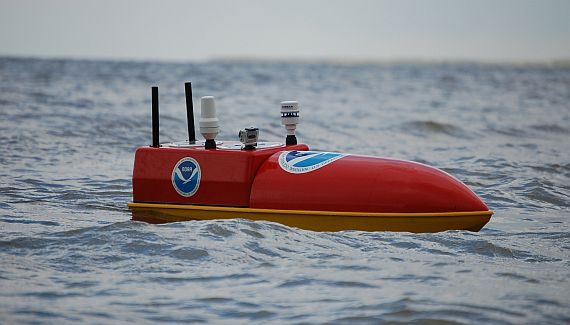
\includegraphics[width=0.6\textwidth,trim={1cm 2cm 1cm 1cm},clip]{img/EMILY_NOAA.jpg}
    \end{center}
\end{frame}

\begin{frame}{Problem Description} \label{PD:missions}
    \begin{block}{Typical USV Missions}
        \begin{columns}
            \begin{column}{0.5\textwidth}
                \begin{block}{}
                    \begin{center}
                        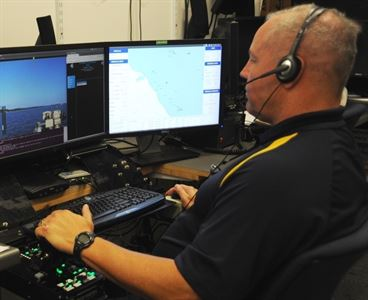
\includegraphics[width=0.85\textwidth]{img/traditional.JPG}
                        \vline
                        \linebreak
                        Remote control
                    \end{center}
                \end{block}
            \end{column}
            \begin{column}{0.5\textwidth}
                \begin{block}{}
                    \begin{center}
                        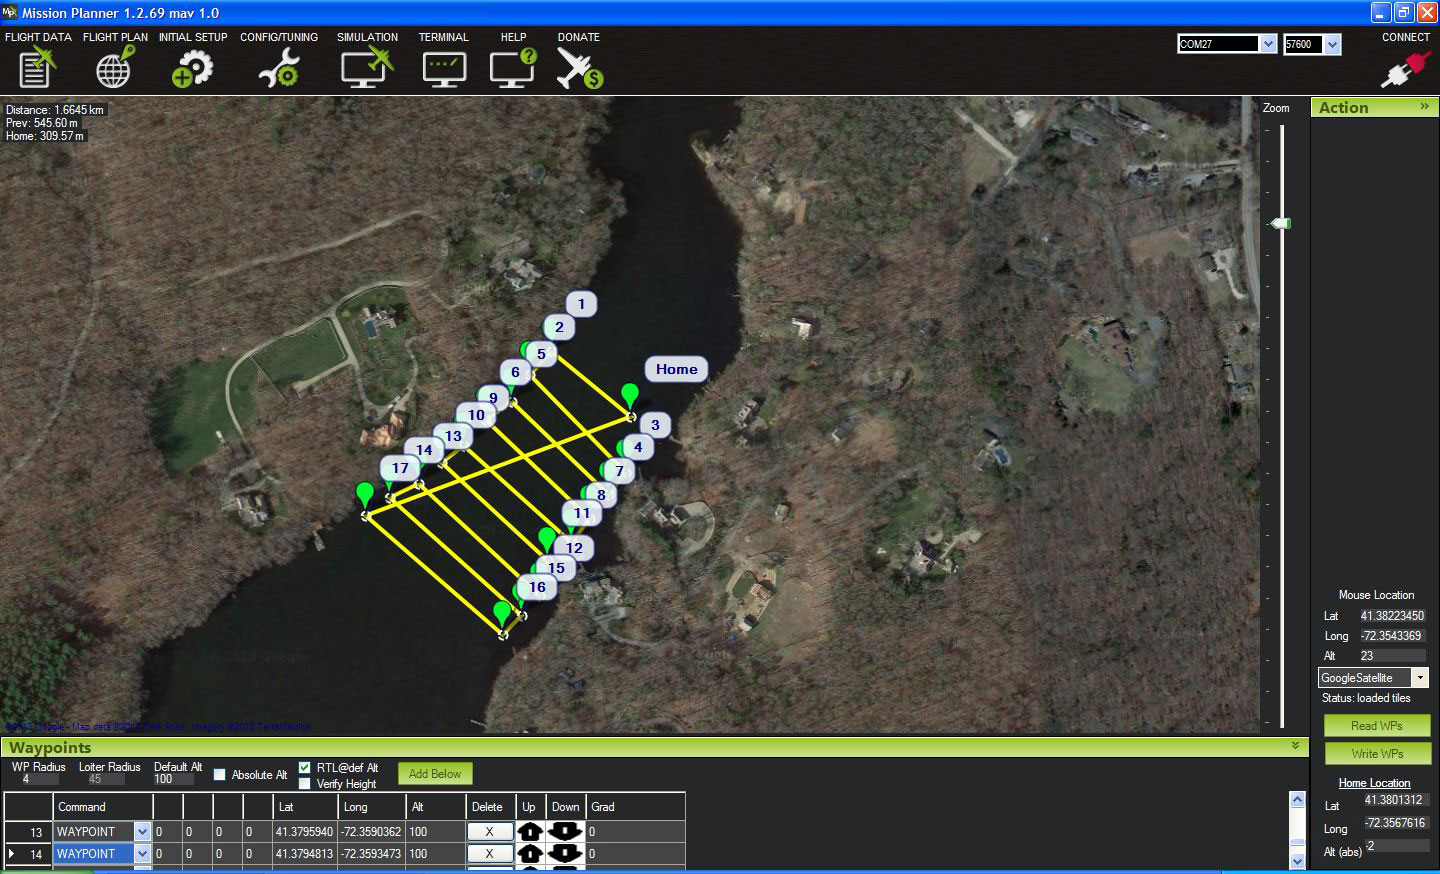
\includegraphics[width=\textwidth,trim={2cm 2cm 8cm 2cm},clip]{img/Jetyak4Waypoints.jpg}
                        \vline
                        \linebreak
                        Manually set waypoints for autopilot
                    \end{center}
                \end{block}
            \end{column}
        \end{columns}
    \end{block}
    \textbf{Goal: from USVs as \textit{tools} to USVs as \textit{agents}}
\end{frame}

\begin{frame}{Problem Description} \label{PD:challenges}
    \begin{block}{Challenges}
	    \begin{itemize}
    	    \item \textbf{Subject to complex dynamic environment}
    	    \item \textbf{Plans with computationally complex algorithms}
	        \item Requires awareness of above and below waterline
	        \item Sensing complicated by platform instability and high noise
    	    \item Must navigate among marine traffic
    	    \item Moves as nonholonomic, dynamic system with large turn radius
    	    \end{itemize}
    \end{block}
    \begin{center}
        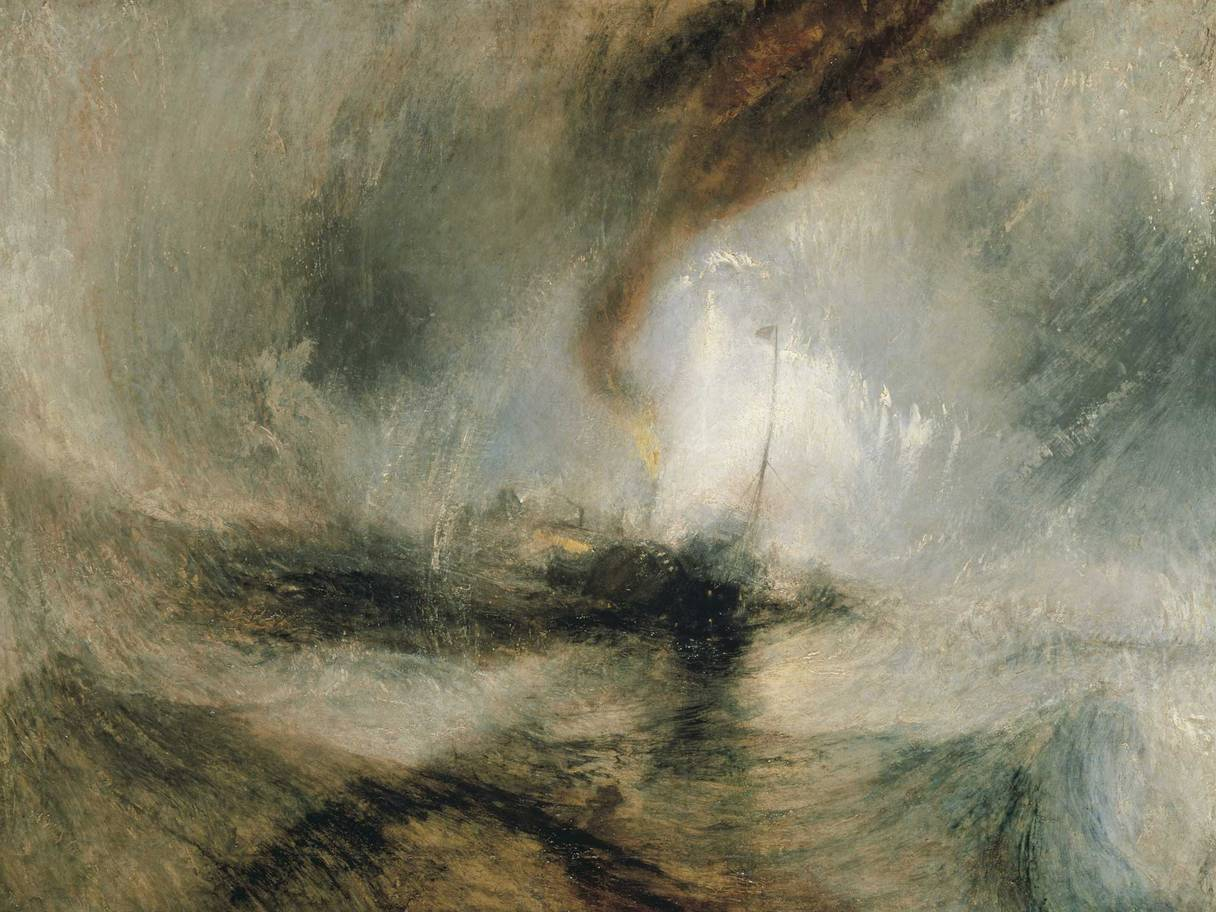
\includegraphics[width=0.5\textwidth,trim={5cm 5cm 4cm 4cm},clip]{img/turner_boat.jpg}
        
        \small{Turner, \textit{Snow Storm --- Steam-Boat off a Harbour’s Mouth}}
    \end{center}
\end{frame}

%%%%%%%%%%%%%%
% Prior Work %
%%%%%%%%%%%%%%
\section{Prior Work} \label{PW:navigation}
\begin{frame}{Prior Work}
    \begin{block}{Autonomous Navigation}
	    \begin{itemize}
    	    \item Guidance, navigation and control is well established with algorithms for path following (such as PurePursuit) and for state estimation (extended Kalman filter)
    	    \item Sensor imagery and reactive behaviors enable collision detection and avoidance
    	    \item Vehicles can be made to follow marine traffic rules and travel in formation
    	    \item Many systems include a \textit{follow} mode that can follow other vehicles, tagged animals, etc
        \end{itemize}
        \begin{columns}
            \begin{column}{0.5\textwidth}
                \begin{center}
                    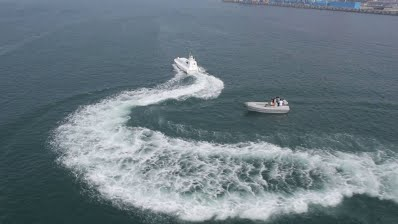
\includegraphics[width=0.65\textwidth,trim={5cm 1cm 2cm 1cm},clip]{img/collisionavoidance.jpg}
                \end{center}
            \end{column}
            \begin{column}{0.5\textwidth}
                \begin{center}
                    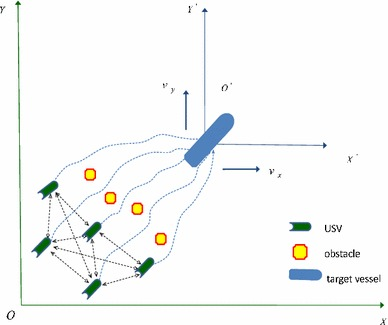
\includegraphics[width=0.65\textwidth,trim={1cm 1cm 4cm 3cm},clip]{img/formation.jpg}
                \end{center}
            \end{column}
        \end{columns}
    \end{block}
\end{frame}

\begin{frame}{Prior Work} \label{PW:planning}
    \begin{columns}
        \begin{column}{0.45\textwidth}
            \begin{block}{Goto Path Planning}
                \begin{center}
                    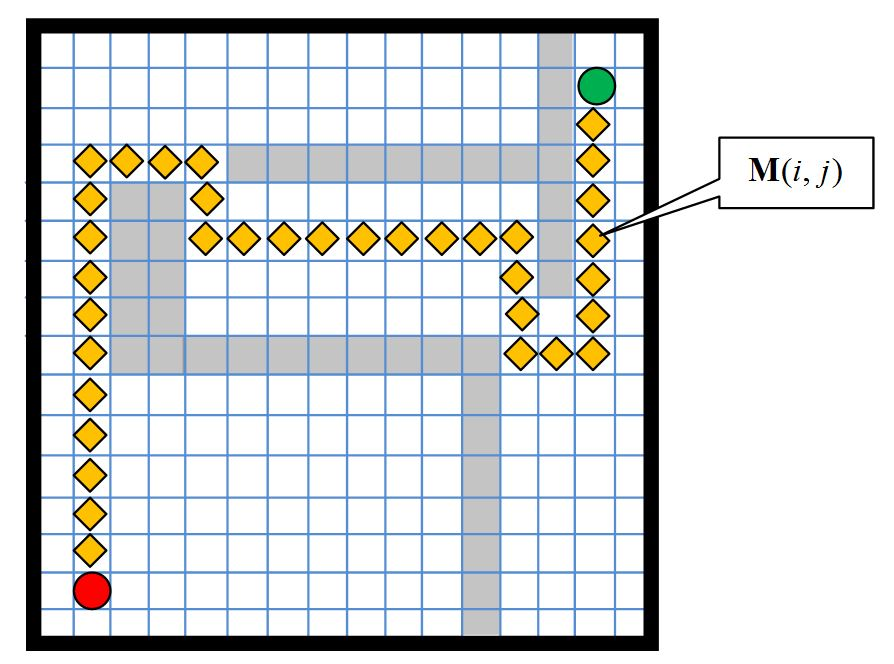
\includegraphics[width=\textwidth,trim={1cm 2cm 5cm 2cm},clip]{img/pathplanning.jpg}
                    \linebreak
                    Computationally complex, even using heuristic and metaheuristic algorithms. 
                    Much work has been done on this problem, but further complicated by dynamic marine environment.
                    Optimizing duration and energy instead of just distance. 
                \end{center}
            \end{block}
        \end{column}
        \begin{column}{0.45\textwidth}
            \begin{block}{Coverage Path Planning}
                \begin{center}
                    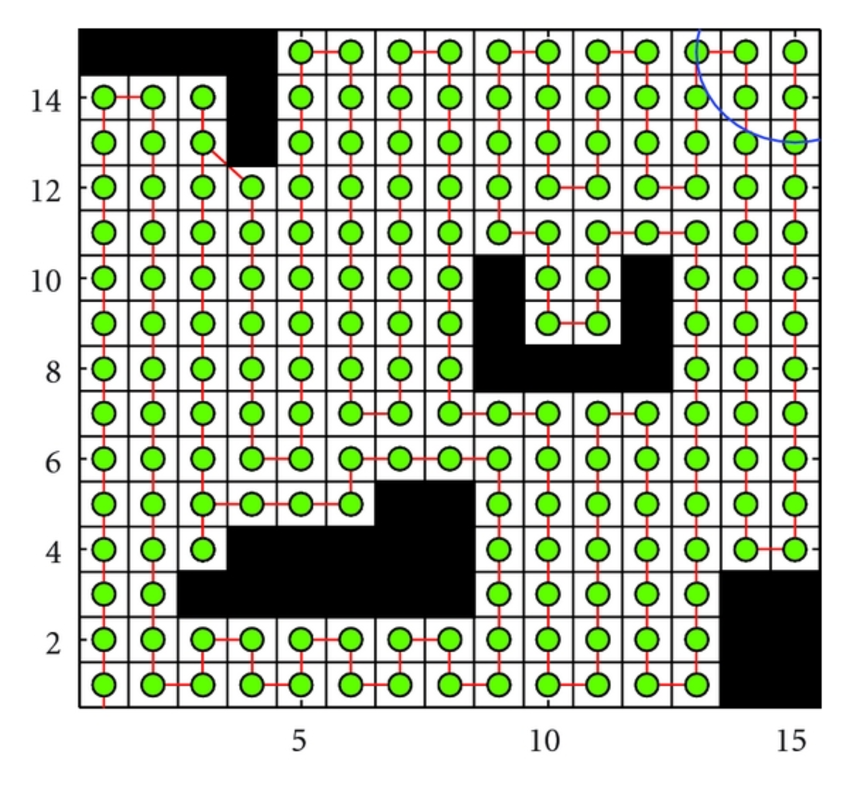
\includegraphics[width=0.85\textwidth,trim={1cm 2cm 2cm 1cm},clip]{img/coverageplanning.png}
                    \linebreak
                    More complicated since (1) a large number of waypoints to solve and (2) maximizing coverage is opposite to minimizing distance. Doing both is especially challenging for heuristic algorithms that may reach a local optimum.
                \end{center}
            \end{block}
        \end{column}
    \end{columns}
\end{frame}

\begin{frame}{Prior Work} 
    \begin{block}{CaRACaS: Control Architecture for Robotic Agent Command and Sensing}
	    \begin{itemize}
	        \item US Navy's platform-agnostic coordinated mission planning system
    	    \item One of few that does onboard mission planning beyond path planning
            \item USVs equipped with the system are part of heterogeneous swarm
	        \item Tasks: Escort ships, protect areas, attack enemy ships
    	    \item Collision detection \& avoidance, COLREGS navigation
    	    \item Able to detect and react to perceived threats
    	    \item Integrated hardware and software
    	    \end{itemize}
    	    
            \small{Michael T. Wolf, et al., "CARACaS multi-agent maritime autonomy for unmanned surface vehicles in the Swarm II harbor patrol demonstration," Proc. SPIE 10195, Unmanned Systems Technology XIX, 101950O (5 May 2017)}

    	    
    \end{block}
\end{frame}  

\begin{frame}{Prior Work} \label{PW:sciencecraft}
    \begin{block}{Autonomous exploration, investigation, and setting objectives}
	    \begin{itemize}
    	    \item Want USV with broad goals such as \textit{investigate Laguna Madre and replan when something interesting detected}
            \item Very little work in this area exists
	        \item Requires reliable mission planning and navigation
        \end{itemize}
        \begin{columns}
            \begin{column}{0.50\textwidth}
                \begin{block}{JPL's Earth Observing-1}
                    \begin{center}
                        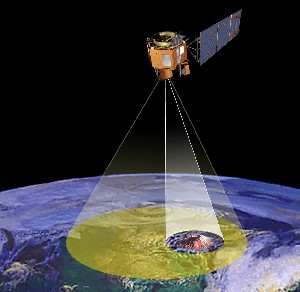
\includegraphics[width=0.65\textwidth,trim={0cm 0cm 0cm 0cm},clip]{img/eo1.jpg}
                    \end{center}
                \end{block}
            \end{column}
            \begin{column}{0.50\textwidth}
                \begin{block}{}
                    \begin{itemize}
        	            \item Onboard analysis: detect image characteristics to such as novel features or sudden change
                        \item Replans to focus on areas of interest
    	                \item Prioritizes interesting data to send to earth first
                    \end{itemize}
                \end{block}
            \end{column}
        \end{columns}
        \small{Sherwood, R.; et al., The Autonomous Sciencecraft Experiment. In IEEE Aerospace Conference (IEEE-Aero 2003), Big Sky, MT, March 2003.}
    \end{block}
\end{frame}  

%%%%%%%%%%%%
% Approach %
%%%%%%%%%%%%
\section{Approach}

\begin{frame}{Approach} \label{A:concept}
    \begin{block}{Concept}
        Rather than a single integrated system, autonomy can be achieved using multiple specialized autonomous agents
    \end{block}
    \begin{columns}
        \begin{column}{0.33\textwidth}
            \begin{block}{Analyst}
                \begin{center}
                    \begin{itemize}
    	                \item Data analysis: detect features \& change
        	            \item Evaluation: assign scientific reward
                        \item Assign targets for \textit{Surveyer} agent
                    \end{itemize}
                    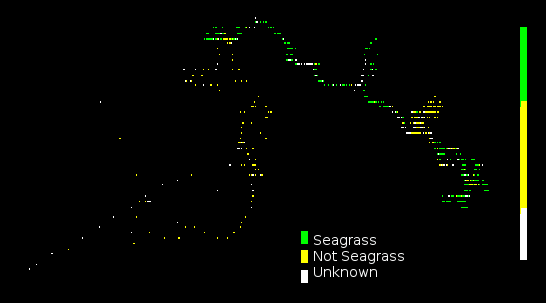
\includegraphics[width=0.75\textwidth,trim={6cm .5cm 4cm .5cm},clip]{img/seagrass.png}
                \end{center}
            \end{block}
        \end{column}
        \begin{column}{0.33\textwidth}
            \begin{block}{Surveyer}
                \begin{center}
                    \begin{itemize}
    	                \item Maximize target reward
        	            \item Collect additional opportunistic reward
                        \item Optimize planning considering complex marine environment
                        \item Ensure vehicle safety
                    \end{itemize}
                    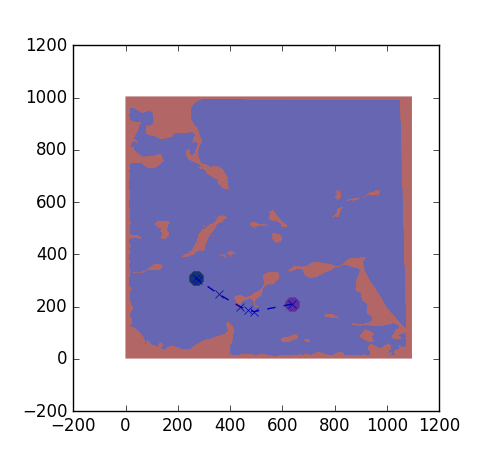
\includegraphics[width=0.75\textwidth,trim={4cm 2cm 4cm 6cm},clip]{img/samplepath.png}
                \end{center}
            \end{block}
        \end{column}
        \begin{column}{0.33\textwidth}
            \begin{block}{Navigator}
                \begin{itemize}
	                \item Path following (mission execution)
    	            \item Collision detection \& avoidance
                    \item Follow COLREGS
	                \item Any issuing of motor commands
                \end{itemize}
                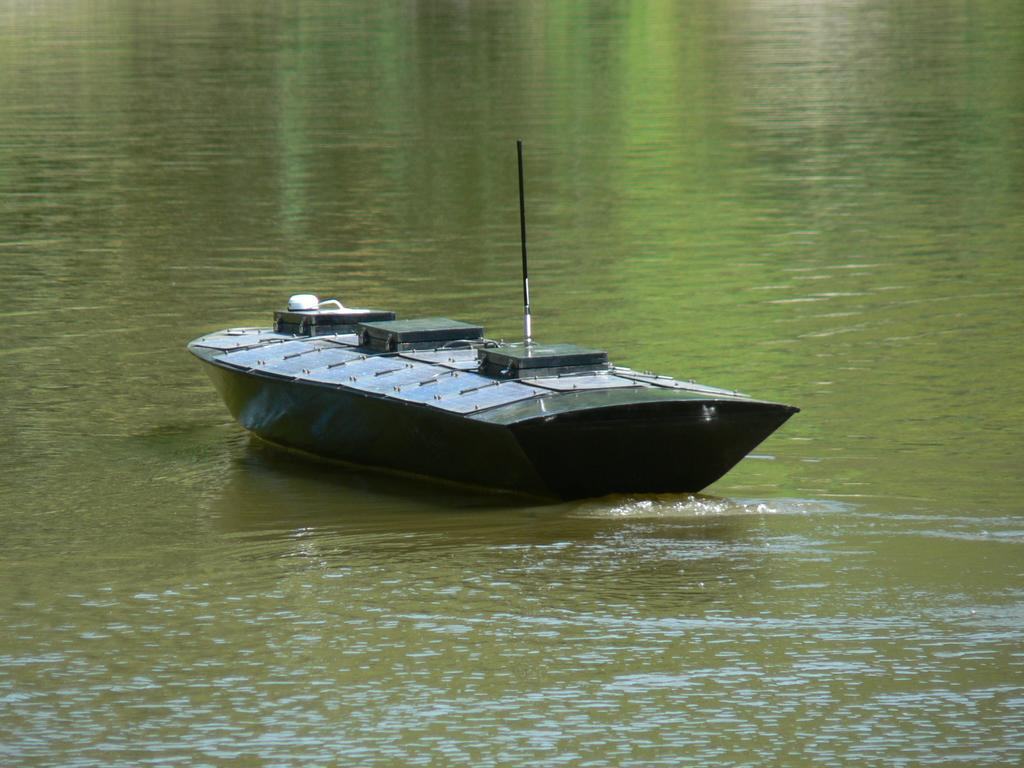
\includegraphics[width=0.75\textwidth,trim={1cm 1cm 1cm 1cm},clip]{img/usv.jpeg}
            \end{block}
        \end{column}
    \end{columns}
\end{frame}  

\begin{frame}{Approach}
    \begin{block}{Heuristics \& Metaheuristics}
        \begin{itemize}
	        \item Analysis and planning techniques are very complex
    	    \item Optimal solutions may take hours or days offline: infeasible online
            \item Human agents able to collect and analyze data without such computations
	        \item \textbf{Heuristic:} using practical measures to achieve a reasonable decision
	        \item \textbf{Metaheuristic:} automatic, indirect heuristic discovery in the form of data-driven, adaptive search strategies
        \end{itemize}
        \begin{center}
            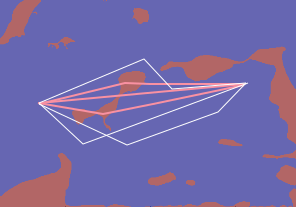
\includegraphics[width=0.5\textwidth,trim={0cm 0cm 0cm 0cm},clip]{img/metaheuristics.png}
        \end{center}
    \end{block}
\end{frame}


%%%%%%%%%%%%%%%%%
% System Design %
%%%%%%%%%%%%%%%%%
\section{System Design}

\begin{frame}{System Design}
    \begin{columns}
        \begin{column}{0.5\textwidth}
            \begin{center}
                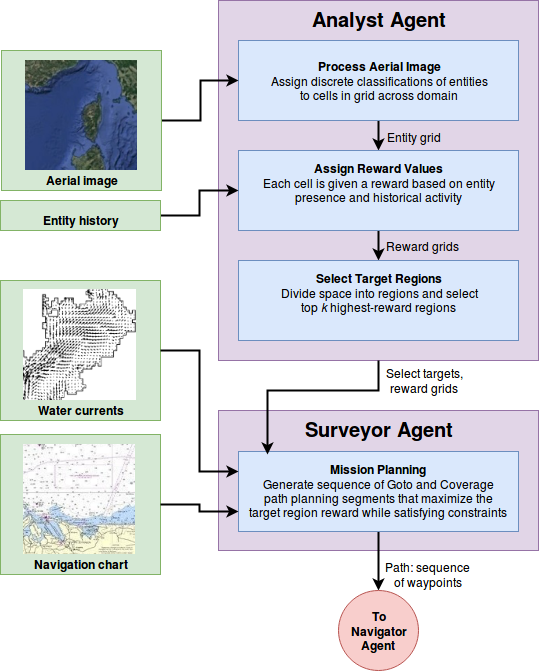
\includegraphics[width=\textwidth,trim={0cm 0cm 0cm 0cm},clip]{img/system_overview.png}
            \end{center}
        \end{column}
        \begin{column}{0.5\textwidth}
            \begin{center}
                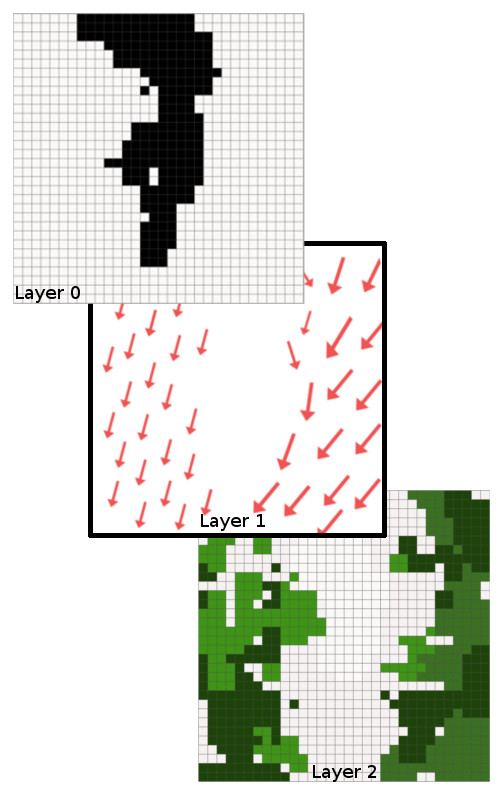
\includegraphics[width=0.75\textwidth,trim={0cm 0cm 0cm 0cm},clip]{img/layers.jpg}
            \end{center}
        \end{column}
    \end{columns}
\end{frame}

\begin{frame}{System Design}
    \begin{block}{Analyst}
        Assigns reward to every cell based on entity presence, speed and acceleration
    \end{block}
    \begin{columns}
        \begin{column}{0.33\textwidth}
            \begin{columns}
                \begin{column}{0.5\textwidth}
                    \begin{center}
                        %\newline
                        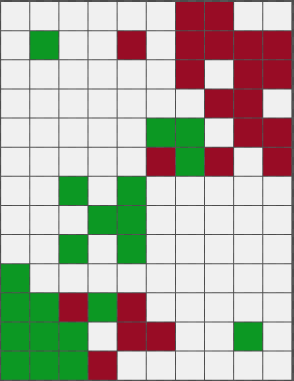
\includegraphics[width=\textwidth,trim={0cm 0cm 0cm 0cm},clip]{img/analyst1.png}
                        \newline
                        Day 1
                        \newline
                        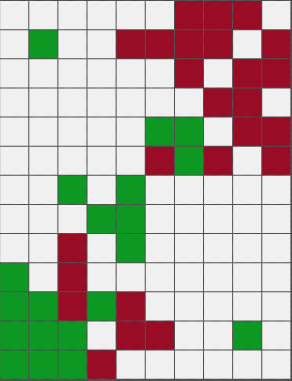
\includegraphics[width=\textwidth,trim={0cm 0cm 0cm 0cm},clip]{img/analyst3.png}
                        \newline
                        Day 3
                    \end{center}
                \end{column}
                \begin{column}{0.5\textwidth}
                    \begin{center}
                        %\newline
                        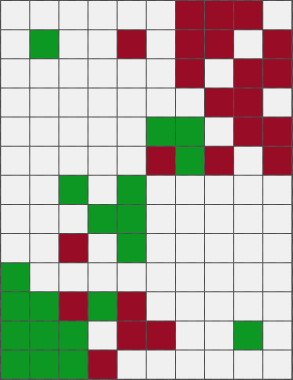
\includegraphics[width=\textwidth,trim={0cm 0cm 0cm 0cm},clip]{img/analyst2.png}
                        \newline
                        Day 2
                        \newline
                        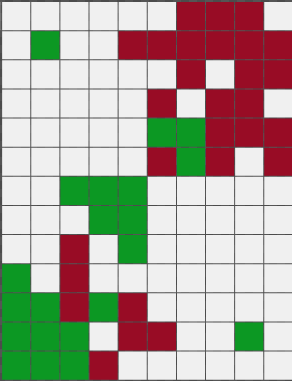
\includegraphics[width=\textwidth,trim={0cm 0cm 0cm 0cm},clip]{img/analyst4.png} 
                        \newline
                        Day 4
                    \end{center}
                \end{column}
            \end{columns}
        \end{column}
        \begin{column}{0.33\textwidth}
            \begin{center}
                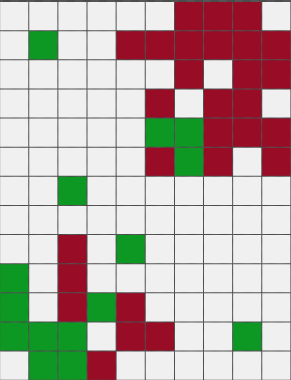
\includegraphics[width=0.50\textwidth,trim={0cm 0cm 0cm 0cm},clip]{img/analyst5.png}
                \newline
                Today's image
                \newline
                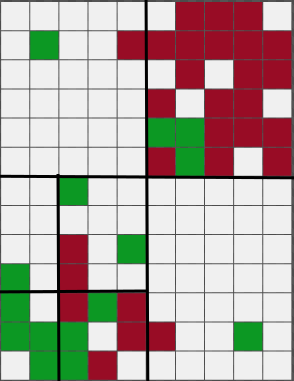
\includegraphics[width=0.50\textwidth,trim={0cm 0cm 0cm 0cm},clip]{img/analyst_grid.png}
                \newline
                Quadtree applied
            \end{center}
        \end{column}
        \begin{column}{0.33\textwidth}
            %\begin{center}
                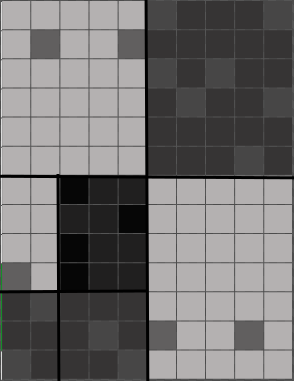
\includegraphics[width=0.50\textwidth,trim={0cm 0cm 0cm 0cm},clip]{img/analyst_grid_2.png}
                \newline
                Reward assignment
                \newline
                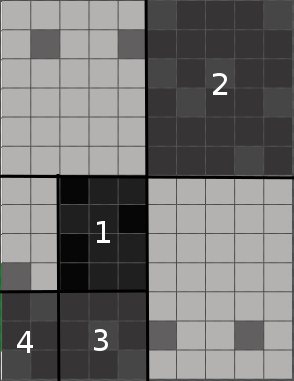
\includegraphics[width=0.50\textwidth,trim={0cm 0cm 0cm 0cm},clip]{img/analyst_grid_targets.png}
                \newline
                Top K targets
            %\end{center}
        \end{column}
    \end{columns}
\end{frame}

\begin{frame}{System Design}
    \begin{block}{Optimality sacrificed for speed}
    \end{block}
    \begin{columns}
        \begin{column}{0.5\textwidth}
            \begin{center}
                \textbf{Quadtree}
                \linebreak
                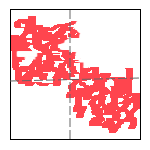
\includegraphics[width=0.75\textwidth,trim={0cm 0cm 0cm 0cm},clip]{img/quadtree_exA.png}
                \begin{itemize}
                        \item Relatively naive
    	                \item Extremely fast
                \end{itemize}
            \end{center}
        \end{column}
        \begin{column}{0.5\textwidth}
            \begin{center}
                \textbf{Optimal}
                \linebreak
                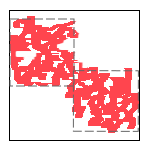
\includegraphics[width=0.75\textwidth,trim={0cm 0cm 0cm 0cm},clip]{img/quadtree_exB.png}
                \begin{itemize}
                        \item Sophisticated reward maximization
    	                \item Very complex
                \end{itemize}  
            \end{center}
        \end{column}
    \end{columns}    
\end{frame}

\begin{frame}{System Design}
    \begin{block}{Surveyor}
        \begin{itemize}
            \item \textbf{Mission planning:} which targets to visit
    	    \item \textbf{\textit{Goto} path planning:} how to get from target to target
    	    \item \textbf{\textit{Coverage} path planning:} how to visit all cells in target region
        \end{itemize}  
    \end{block}
    \begin{columns}
        \begin{column}{0.5\textwidth}
            \begin{center}
                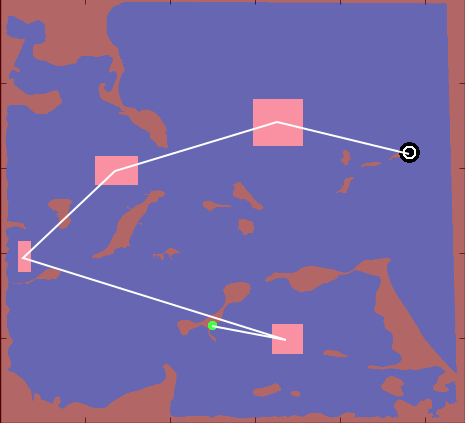
\includegraphics[width=0.75\textwidth,trim={0cm 0cm 0cm 0cm},clip]{img/surveyor_1.png}
                \newline
                Selected target order
            \end{center}
        \end{column}
        \begin{column}{0.5\textwidth}
            \begin{center}
                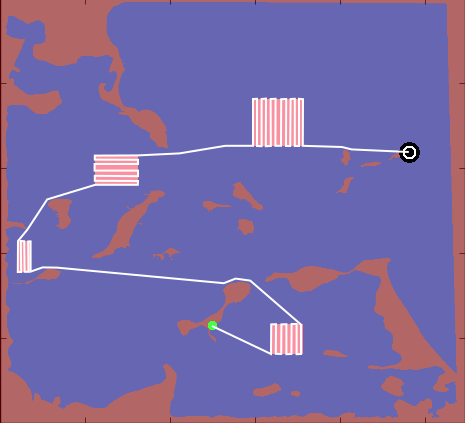
\includegraphics[width=0.75\textwidth,trim={0cm 0cm 0cm 0cm},clip]{img/surveyor_2.png}
                \newline
                \textit{Goto} and \textit{Coverage} paths
            \end{center}
        \end{column}
    \end{columns}
\end{frame}


\begin{frame}{System Design}
    \begin{block}{\textit{Goto} Planning}
        \begin{itemize}
	        \item Optimal is to solve Traveling Salesman Problem (NP-hard)
    	    \item Heuristics are the norm: \textit{A*}, \textit{Potential Field}, \textit{Voronoi Diagram} \newline Still complex for such large regions
            \item Metaheuristics increasingly common: \textit{Genetic Algorithm}, \textit{Particle Swarm Optimization} \newline But non-deterministic and not guaranteed to converge
	        \item Surveyor has to balance opposing criteria
	        \begin{itemize}
	            \item Efficiency: minimize distance, duration, and energy
	            \item Opportunity: maximize reward
	        \end{itemize}
	        \item This work uses metaheuristics. Has to show: 
	        \begin{itemize}
	            \item Approximate optimality
	            \item Acceptable speed and reliability of convergence
	            \item Planning can be modified for a desired behavior
	        \end{itemize}
        \end{itemize}
        %\begin{center}
        %    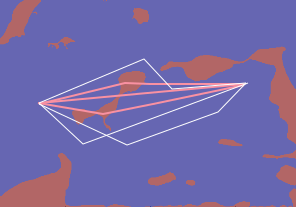
\includegraphics[width=0.5\textwidth,trim={0cm 0cm 0cm 0cm},clip]{img/metaheuristics.png}
        %\end{center}
    \end{block}
\end{frame}

\begin{frame}{System Design}
    \begin{block}{Metaheuristic \textit{Goto} Planning}
        Which algorithm to use? 
	    \begin{itemize}
	        \item Evolutionary approach
	        \begin{itemize}
	            \item Genetic Algorithm (GA)
	            \item Differential Evolution (DE)
	        \end{itemize}
	        \item Colony behavior approach
	        \begin{itemize}
	            \item Particle Swarm Optimization (PSO)
	            \item Artificial Bee Colony (ABC)
	        \end{itemize}
        \end{itemize}
    \end{block}
    \begin{columns}
         \begin{column}{0.5\textwidth}
             \begin{block}{Evolutionary approach}   
                 \begin{center}
                     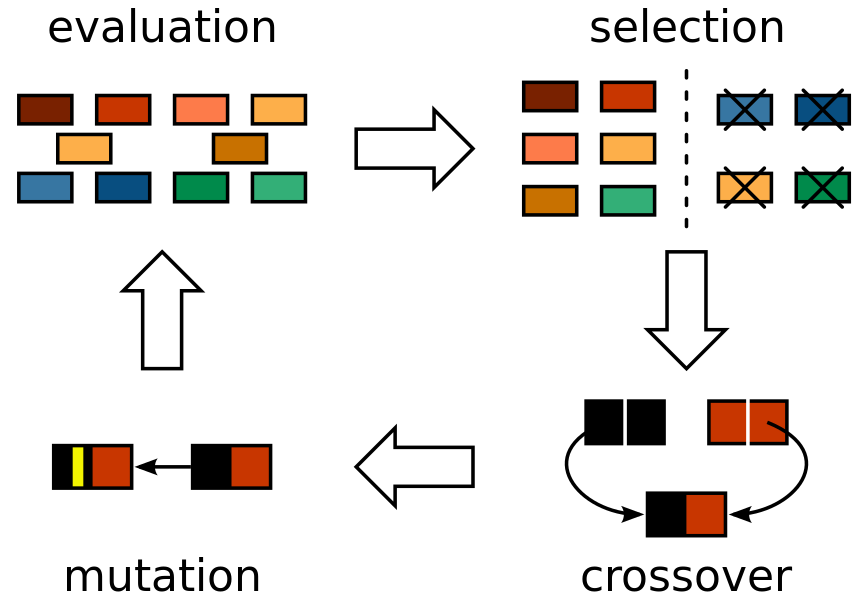
\includegraphics[width=0.8\textwidth,trim={0cm 0cm 0cm 0cm},clip]{img/ga.png}
                 \end{center}
             \end{block} 
        \end{column}
        \begin{column}{0.5\textwidth}
             \begin{block}{Colony behavior approach}   
                 \begin{center}
                     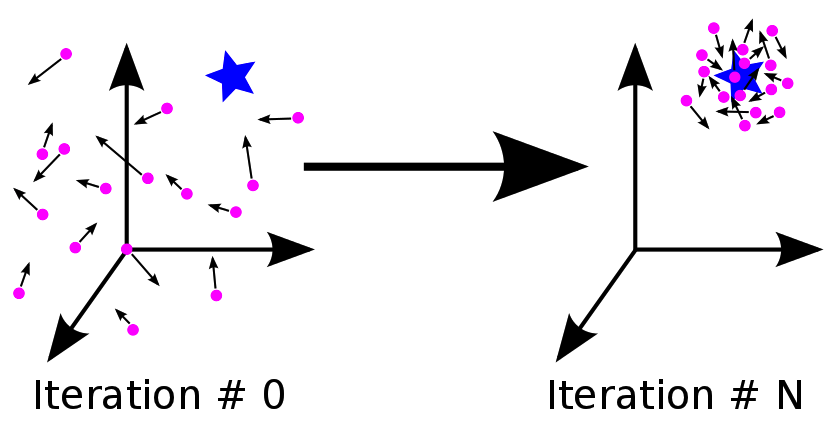
\includegraphics[width=\textwidth,trim={0cm 0cm 0cm 0cm},clip]{img/pso.png}
                 \end{center}
             \end{block} 
        \end{column}
    \end{columns}
\end{frame}

\begin{frame}{System Design} \label{SD:metaheuristic}
    \begin{block}{Metaheuristic \textit{Goto} Planning fitness function}
	    \begin{itemize}
	        \item Evaluates an ordered sequence of (row, column) waypoints
	        \item Each cell on the line between each waypoint is evaluated
	        \item Considers multiple weighted criteria
	        \begin{itemize}
	            \item \textbf{Collisions:} number of obstacle cells encountered
	            \item \textbf{Distance:} distance between waypoints
	            \item \textbf{Energy:} applied work done to traverse cell at desired speed and heading
	            \item \textbf{Reward:} reward value at each cell
	        \end{itemize}
	        \item Duration estimate required to index closest temporal water currents forecast
        \end{itemize}
    \end{block}

    \begin{columns}
         \begin{column}{0.33\textwidth}
             \begin{block}{Region}   
                 \begin{center}
                     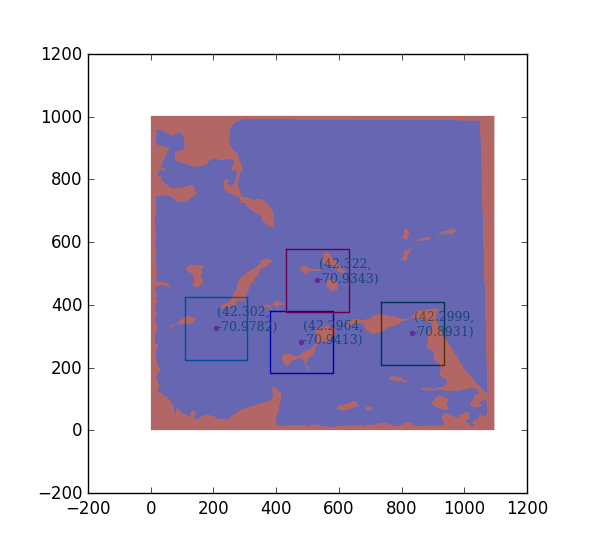
\includegraphics[width=0.8\textwidth,trim={3cm 3cm 3cm 3cm},clip]{img/Fig_targetsMap.png}
                 \end{center}
             \end{block} 
        \end{column}
        \begin{column}{0.33\textwidth}
             \begin{block}{Water currents}   
                 \begin{center}
                     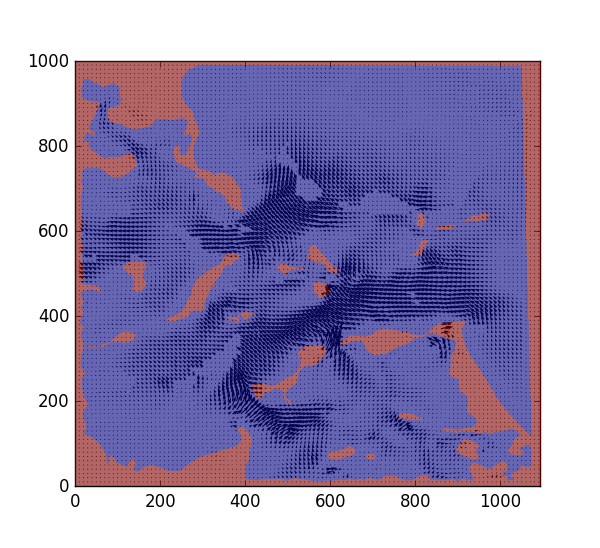
\includegraphics[width=0.75\textwidth,trim={2cm 2cm 1.75cm 1cm},clip]{img/Fig_currentsMap-1.png}
                 \end{center}
             \end{block} 
        \end{column}
         \begin{column}{0.33\textwidth}
             \begin{block}{Entities}   
                 \begin{center}
                     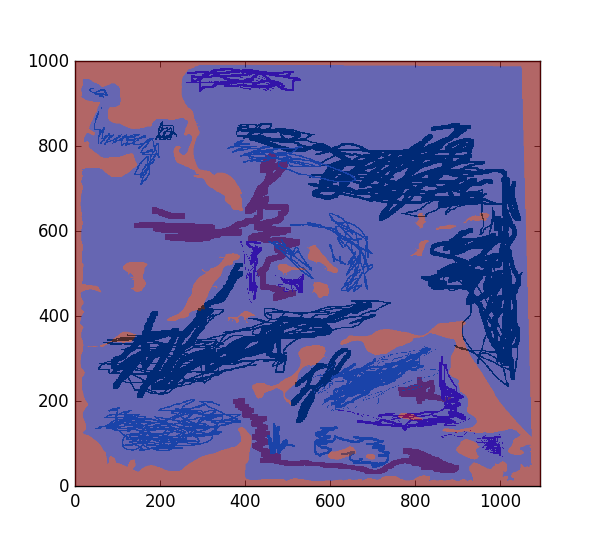
\includegraphics[width=0.75\textwidth,trim={2cm 2cm 1.75cm 1cm},clip]{img/Fig_entitiesMap.png}
                 \end{center}
             \end{block} 
        \end{column}
    \end{columns}
\end{frame}


\begin{frame}{System Design}
    \begin{block}{\textit{Coverage} Path Planning}
	    \begin{itemize}
	        \item Visit each cell (or sample a percentage of cells)
	        \item Existence of obstacles greatly increases planning complexity
	        \item Feasibility constrained by maximum duration and energy
	        \item \textbf{No obstacles:} lawnmower path
	        \item \textbf{Has obstacles:} A work in progress... 
        \end{itemize}
    \end{block}

    \begin{columns}
         \begin{column}{0.45\textwidth}
             \begin{block}{Column-wise}   
                 \begin{center}
                     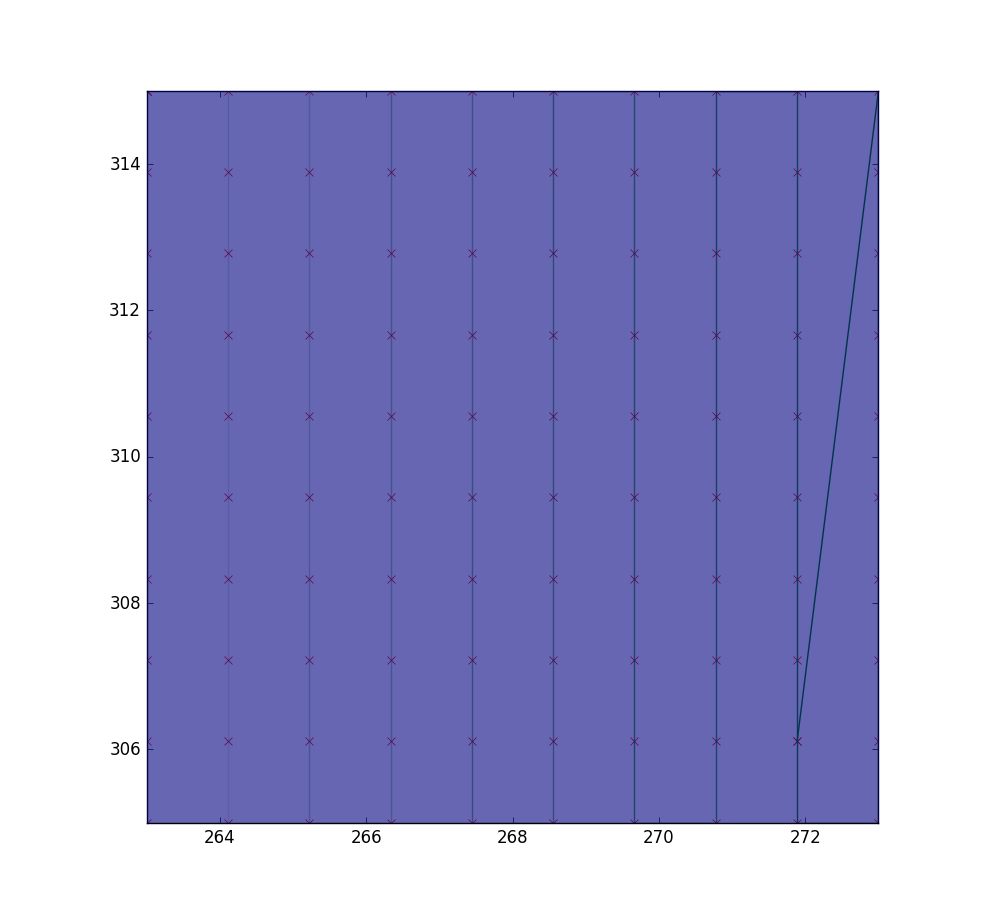
\includegraphics[width=0.8\textwidth,trim={4cm 3cm 0cm 0cm},clip]{img/EXP2RC1-0_col.png}
                 \end{center}
             \end{block} 
        \end{column}
        \begin{column}{0.45\textwidth}
             \begin{block}{Row-wise}   
                 \begin{center}
                     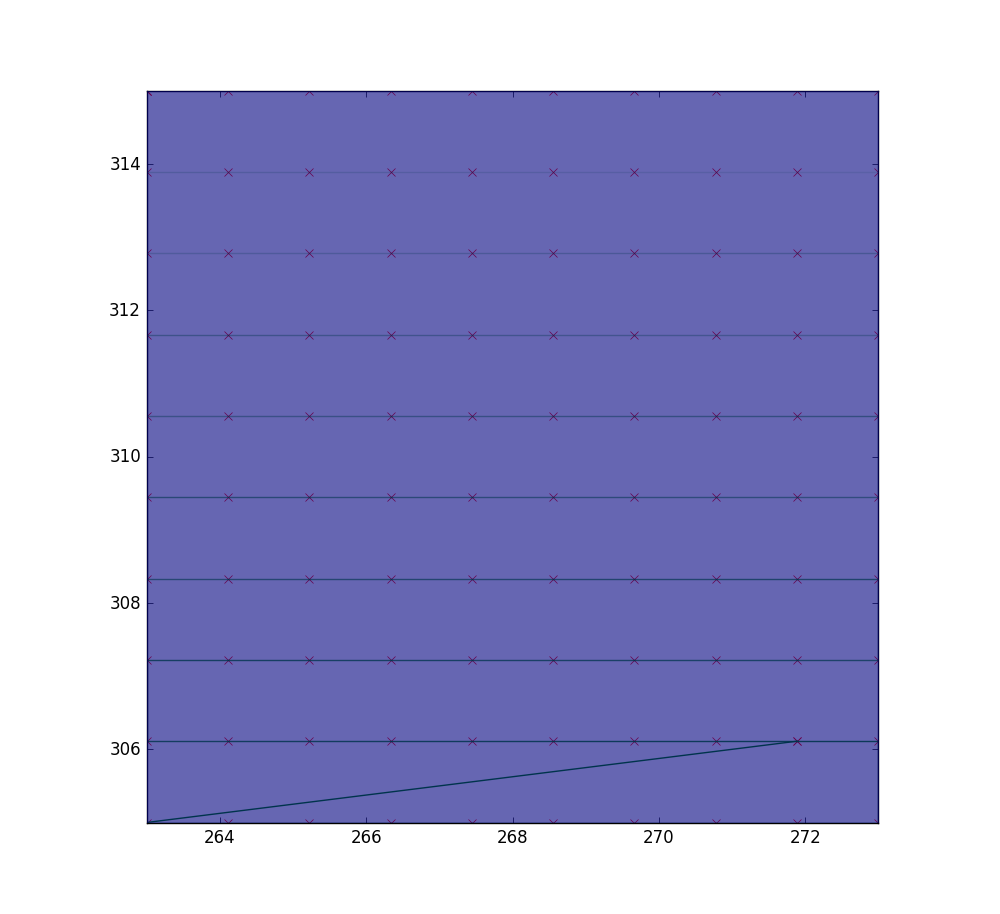
\includegraphics[width=0.8\textwidth,trim={4cm 3cm 0cm 0cm},clip]{img/EXP2RC1-0_row.png}
                 \end{center}
             \end{block} 
        \end{column}
    \end{columns}
\end{frame}

\begin{frame}{System Design}
    \begin{block}{Mission Planning}
	    \begin{itemize}
	        \item Find best feasible sequence to visit targets
	        \item Dynamic environment: time matters 
	        \item Target region entrance and exit points matter
	        \item Feasibility constrained by maximum duration and energy
        \end{itemize}
    \end{block}
    \begin{block}{Possible mission}
        \begin{center}
            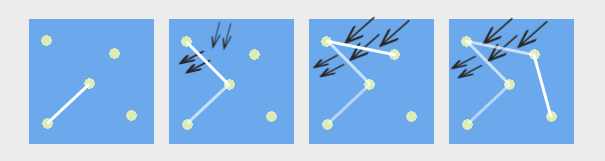
\includegraphics[width=0.75\textwidth,trim={1cm 1cm 1cm 1cm},clip]{img/mission_planning_planA.png}
        \end{center}
    \end{block}
    \begin{block}{Lower energy cost alternative}
        \begin{center}
            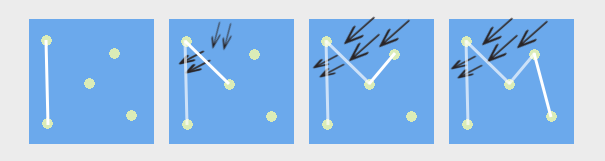
\includegraphics[width=0.75\textwidth,trim={1cm 1cm 1cm 1cm},clip]{img/mission_planning_planB.png}
        \end{center}
    \end{block}
\end{frame}

\begin{frame}{System Design}
    \begin{block}{Mission Planning: complexity concerns}
	    \begin{itemize}
	        \item Suppose you have $N$ targets and $S$ allowed stop locations
	        \item Large number of missions to evaluate: $N! \times S$
	        \item A maximal mission has $N + 1$ \textit{Goto} paths and $N$ \textit{Coverage} paths
	        \item Memoization limited by dependency on elapsed duration and target region exit \& entry points
	        \item \textbf{Goal:} Find a heuristic to limit the search space
        \end{itemize}
    \end{block}
    \begin{center}
        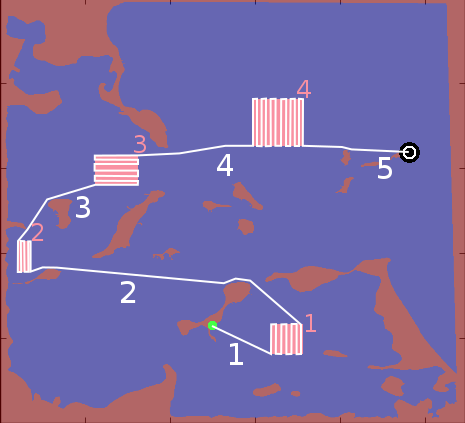
\includegraphics[width=0.5\textwidth,trim={0cm 1cm 0cm 1.75cm},clip]{img/nummissions.png}
    \end{center}
\end{frame}

%%%%%%%%%%%%%%
% Evaluation %
%%%%%%%%%%%%%%
\section{Evaluation}
\begin{frame}{Evaluation}
    \begin{block}{Research questions}
	    \begin{itemize}
	        \item Is using metaheuristic algorithms for \textit{Goto} planning effective despite the addition of reward maximization? Do we see acceptable convergence and repeatibility?
	        \item Which metaheuristic algorithm to use out of the four candidates? Do they differ significantly?
	        \item Can the weights on work and reward criteria be set to achieve a desired planning behavior?
	        \item Does the impact of dynamic marine environment affect planning?
	        \item Can mission planning be done without exhaustive search?
        \end{itemize}
    \end{block}
\end{frame}

\begin{frame}{Evaluation}
    \begin{columns}
        \begin{column}{0.5\textwidth}
            \begin{center}
                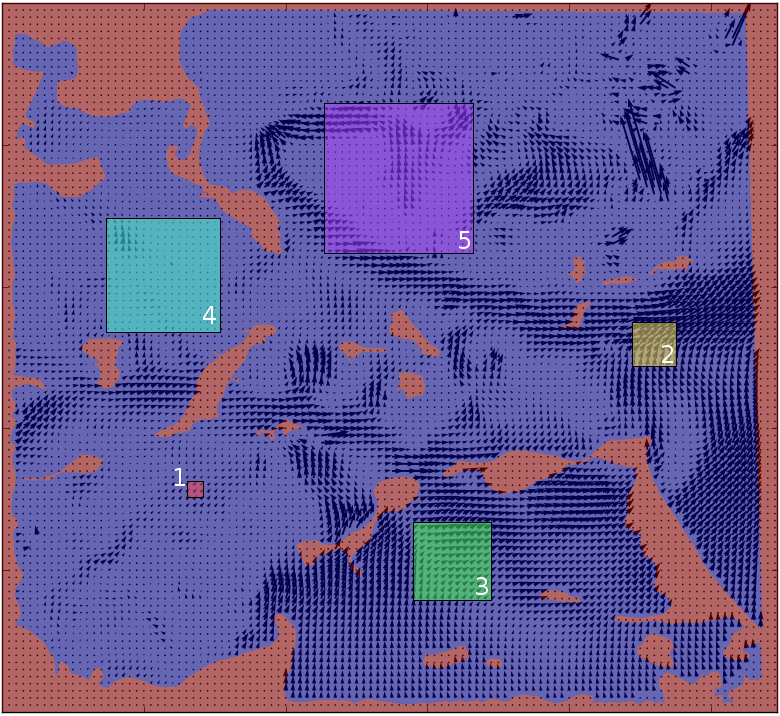
\includegraphics[width=\textwidth,trim={0cm 1cm 0cm 1.75cm},clip]{img/CurrentsTargetMap.png}
            \end{center}
        \end{column}
        \begin{column}{0.5\textwidth}
            \begin{block}{Experimental environment}
        	    \begin{itemize}
        	        \item Massachusetts Bay has 48-hour models: source of water current forecasts
        	        \item Five targets selected of increasing size
        	        \item Targets intentionally places to see effect of water currents and terrain avoidance
        	        \item Maximum duration and energy set to \textit{very high} so that a feasible mission can complete all targets
        	        \item Water current forecasts update in 30 minute intervals
                \end{itemize}
            \end{block}
        \end{column}
    \end{columns}
\end{frame}

\begin{frame}{Evaluation}
    \begin{block}{Initial \textit{Goto} results using PSO (Direction \textbf{A})}
        \begin{columns}
            \begin{column}{0.25\textwidth}
                \begin{center}
                        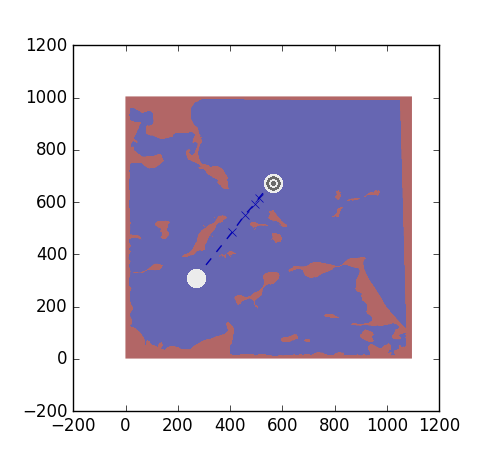
\includegraphics[width=\textwidth,trim={2cm 2cm 2cm 2cm},clip]{img/EXP3RG_PathAa_-1_-1_0_0.png}
                \end{center}
            \end{column}
            \begin{column}{0.25\textwidth}
                \begin{center}
                    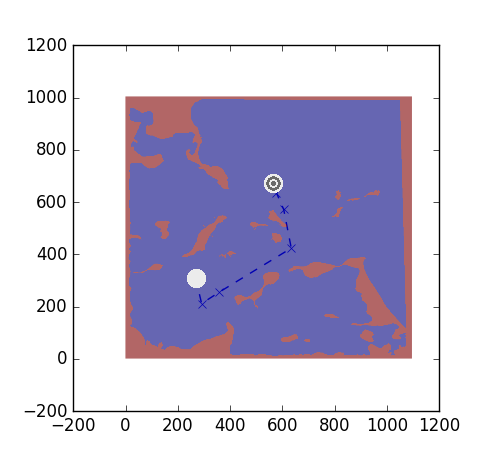
\includegraphics[width=\textwidth,trim={2cm 2cm 2cm 2cm},clip]{img/EXP3RG_PathAa_-1_-1_0_-1.png}
                \end{center}
            \end{column}
            \begin{column}{0.25\textwidth}
                \begin{center}
                    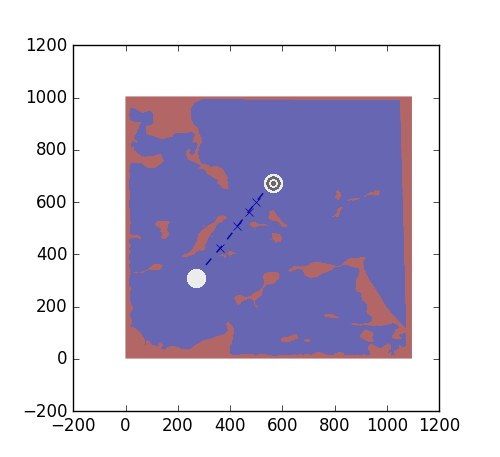
\includegraphics[width=\textwidth,trim={2cm 2cm 2cm 2cm},clip]{img/EXP3RG_PathAa_-1_-1_-1_0.png}
                \end{center}
            \end{column}
            \begin{column}{0.25\textwidth}
                \begin{center}
                    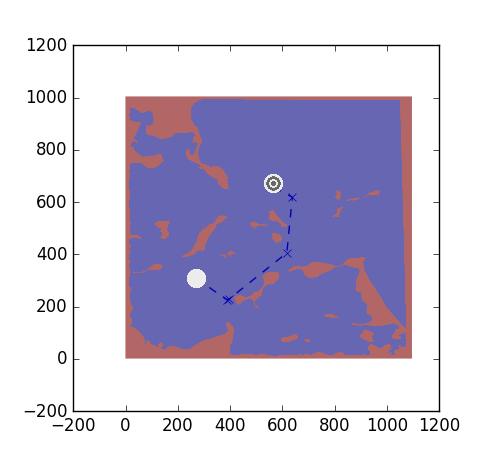
\includegraphics[width=\textwidth,trim={2cm 2cm 2cm 2cm},clip]{img/EXP3RG_PathAa_-1_-1_-1_-1.png}
                \end{center}
            \end{column}
        \end{columns}
    \end{block}
    \begin{block}{Initial \textit{Goto} results using PSO (Direction \textbf{B})}
        \begin{columns}
            \begin{column}{0.25\textwidth}
                \begin{center}
                        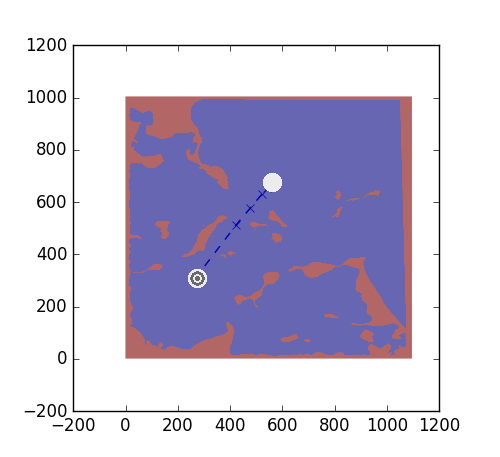
\includegraphics[width=\textwidth,trim={2cm 2cm 2cm 2cm},clip]{img/EXP3RG_PathAb_-1_-1_0_0.png}
                \end{center}
            \end{column}
            \begin{column}{0.25\textwidth}
                \begin{center}
                    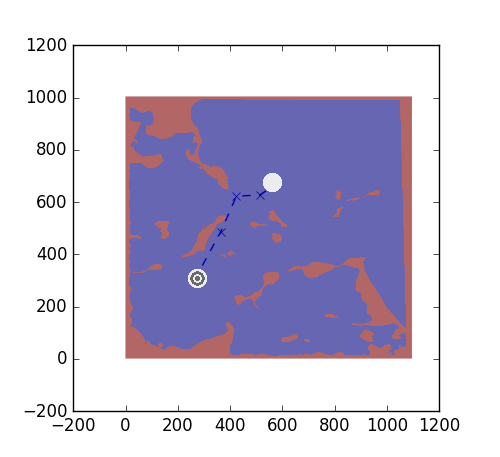
\includegraphics[width=\textwidth,trim={2cm 2cm 2cm 2cm},clip]{img/EXP3RG_PathAb_-1_-1_0_-1.png}
                \end{center}
            \end{column}
            \begin{column}{0.25\textwidth}
                \begin{center}
                    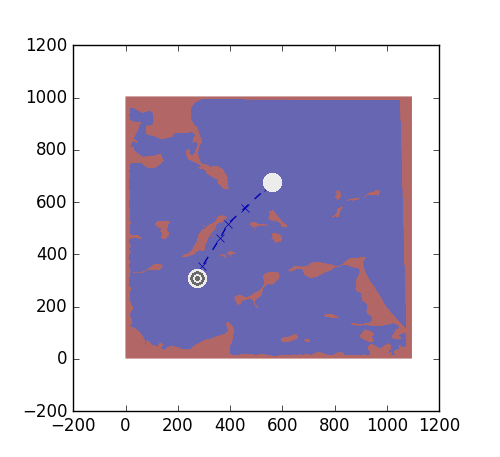
\includegraphics[width=\textwidth,trim={2cm 2cm 2cm 2cm},clip]{img/EXP3RG_PathAb_-1_-1_-1_0.png}
                \end{center}
            \end{column}
            \begin{column}{0.25\textwidth}
                \begin{center}
                    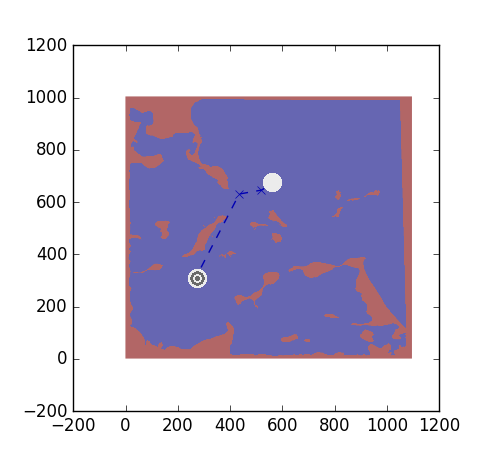
\includegraphics[width=\textwidth,trim={2cm 2cm 2cm 2cm},clip]{img/EXP3RG_PathAb_-1_-1_-1_-1.png}
                \end{center}
            \end{column}
        \end{columns}
    \end{block}
\end{frame}

\begin{frame}{Evaluation}
    \begin{block}{Comparison of metaheuristic \textit{Goto} planning}
    \small{Note: all algorithms have same execution time for each iteration}
    \end{block}
    \begin{block}{Particle swarm optimization}
        \begin{columns}
            \begin{column}{0.5\textwidth}
                \begin{center}
                    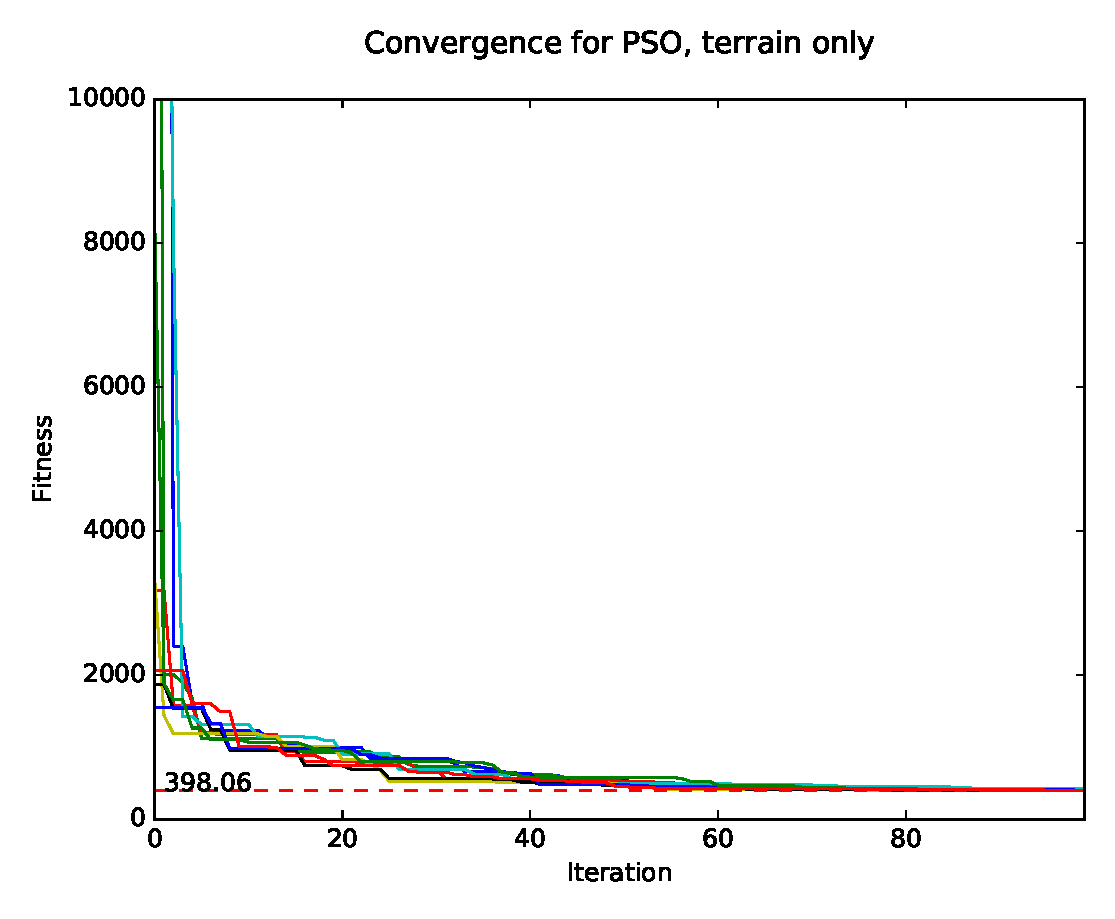
\includegraphics[width=\textwidth,trim={.75cm .75cm 0cm 1cm},clip]{img/conv_PSO_a.eps}
                    \linebreak
                    terrain, distance
                \end{center}
            \end{column}
            \begin{column}{0.5\textwidth}
                \begin{center}
                    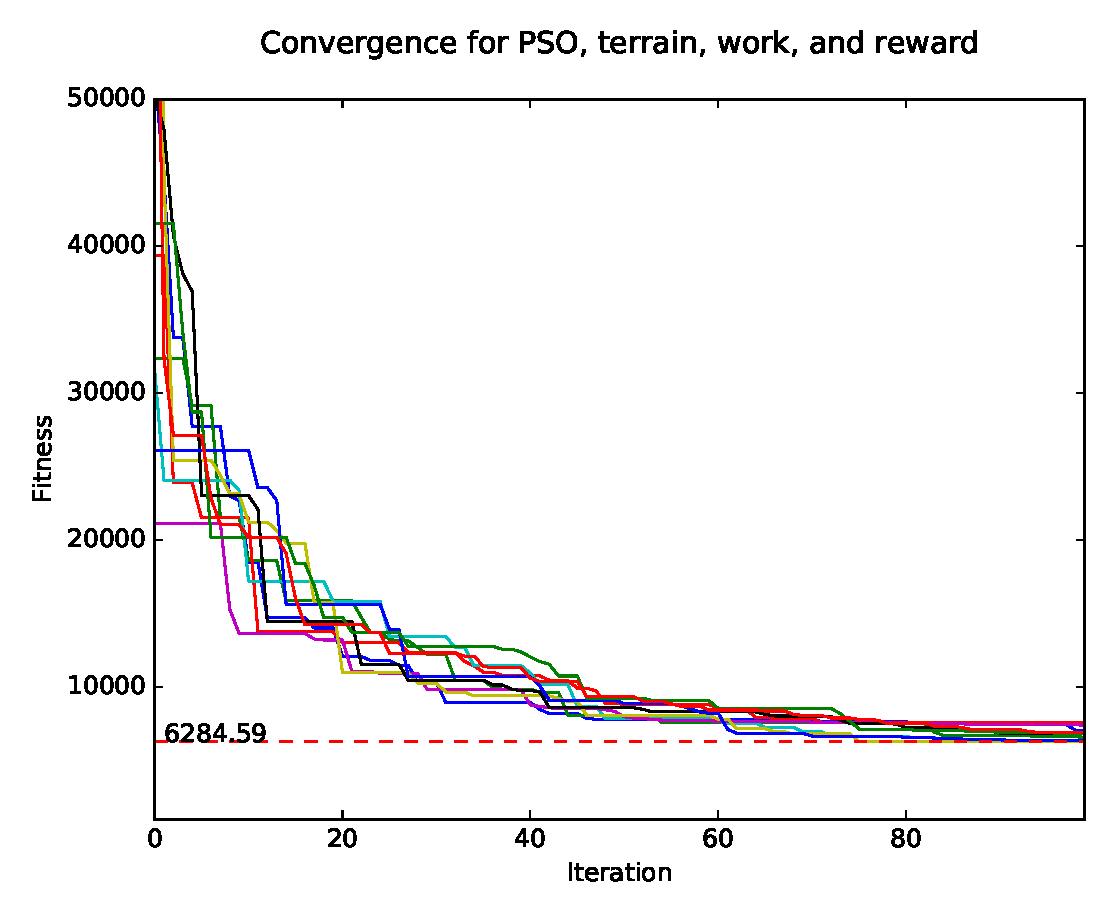
\includegraphics[width=\textwidth,trim={.75cm .75cm 0cm 1cm},clip]{img/conv_PSO_b.eps}
                    \linebreak
                    terrain, distance, energy, reward
                \end{center}
            \end{column}
        \end{columns}
    \end{block}
\end{frame}

\begin{frame}{Evaluation}
    \begin{block}{Comparison of metaheuristic \textit{Goto} planning}
    \end{block}
    \begin{block}{Genetic algorithm}
        \begin{columns}
            \begin{column}{0.5\textwidth}
                \begin{center}
                    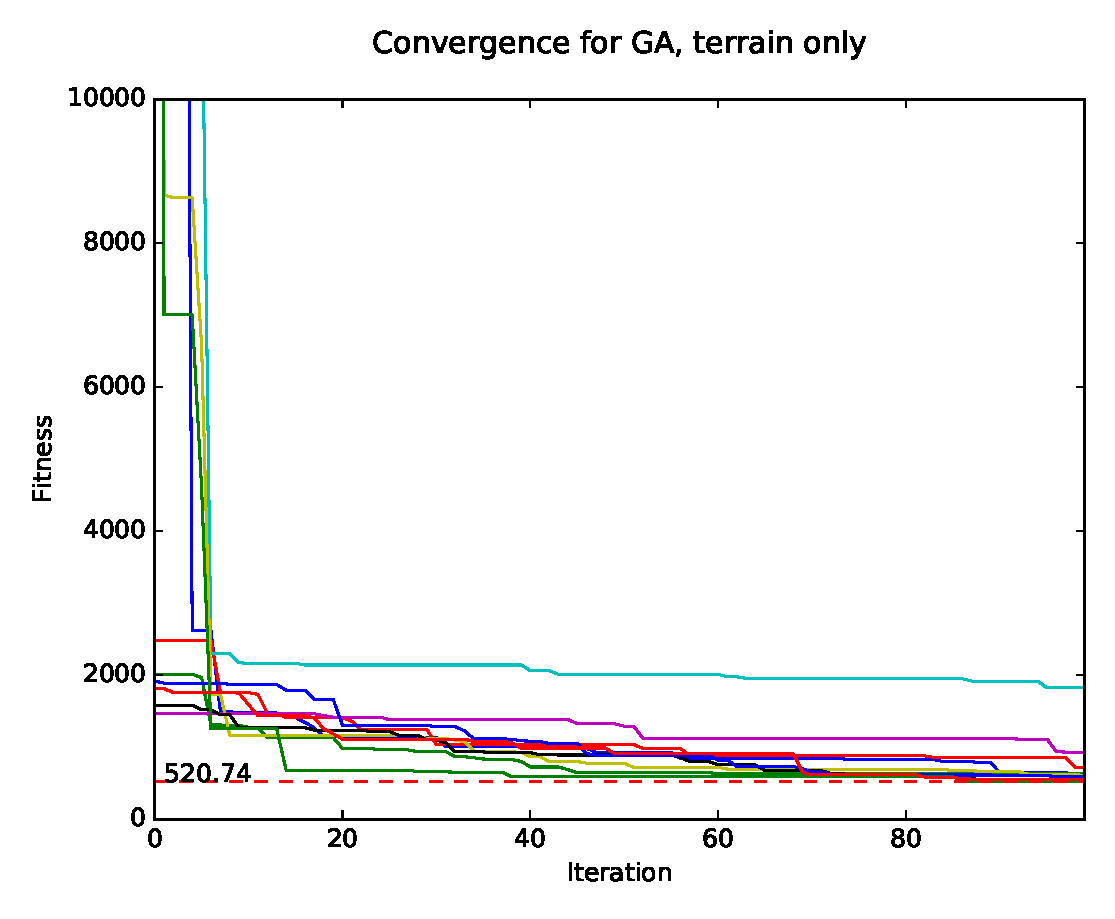
\includegraphics[width=\textwidth,trim={.75cm .75cm 0cm 1cm},clip]{img/conv_GA_a.eps}
                    \linebreak
                    terrain, distance
                \end{center}
            \end{column}
            \begin{column}{0.5\textwidth}
                \begin{center}
                    \includegraphics[width=\textwidth,trim={.75cm .75cm 0cm 1cm},clip]{img/conv_GA_b.eps}
                    \linebreak
                    terrain, distance, energy, reward
                \end{center}
            \end{column}
        \end{columns}
    \end{block}
\end{frame}

\begin{frame}{Evaluation}
    \begin{block}{Comparison of metaheuristic \textit{Goto} planning}
    \end{block}
    \begin{block}{Artificial bee colony}
        \begin{columns}
            \begin{column}{0.5\textwidth}
                \begin{center}
                    \includegraphics[width=\textwidth,trim={.75cm .75cm 0cm 1cm},clip]{img/conv_BEE_a.eps}
                    \linebreak
                    terrain, distance
                \end{center}
            \end{column}
            \begin{column}{0.5\textwidth}
                \begin{center}
                    \includegraphics[width=\textwidth,trim={.75cm .75cm 0cm 1cm},clip]{img/conv_BEE_b.eps}
                    \linebreak
                    terrain, distance, energy, reward
                \end{center}
            \end{column}
        \end{columns}
    \end{block}
\end{frame}

\begin{frame}{Evaluation}
    \begin{block}{Comparison of metaheuristic \textit{Goto} planning}
    \end{block}
    \begin{block}{Differential evolution}
        \begin{columns}
            \begin{column}{0.5\textwidth}
                \begin{center}
                    \includegraphics[width=\textwidth,trim={.75cm .75cm 0cm 1cm},clip]{img/conv_DE_a.eps}
                    \linebreak
                    terrain, distance
                \end{center}
            \end{column}
            \begin{column}{0.5\textwidth}
                \begin{center}
                    \includegraphics[width=\textwidth,trim={.75cm .75cm 0cm 1cm},clip]{img/conv_DE_b.eps}
                    \linebreak
                    terrain, distance, energy, reward
                \end{center}
            \end{column}
        \end{columns}
    \end{block}
\end{frame}

\begin{frame}{Evaluation}
    \begin{block}{Comparison of metaheuristic \textit{Goto} planning}
    \end{block}
    \begin{block}{Average curves}
        \begin{columns}
            \begin{column}{0.5\textwidth}
                \begin{center}
                    \includegraphics[width=\textwidth,trim={.75cm .75cm 0cm 1cm},clip]{img/conv_avg_a.eps}
                    \linebreak
                    terrain, distance
                \end{center}
            \end{column}
            \begin{column}{0.5\textwidth}
                \begin{center}
                    \includegraphics[width=\textwidth,trim={.75cm .75cm 0cm 1cm},clip]{img/conv_avg_b.eps}
                    \linebreak
                    terrain, distance, energy, reward
                \end{center}
            \end{column}
        \end{columns}
    \end{block}
\end{frame}


\begin{frame}{Evaluation}
    \begin{block}{Comparison of metaheuristic \textit{Goto} planning}
    \end{block}
    \begin{block}{Distribution of path distance}
        \begin{columns}
            \begin{column}{0.5\textwidth}
                \begin{center}
                    \includegraphics[width=\textwidth,trim={.75cm .75cm 0cm 1cm},clip]{img/EXP3_histo_distance_a.eps}
                    \linebreak
                    terrain, distance
                \end{center}
            \end{column}
            \begin{column}{0.5\textwidth}
                \begin{center}
                    \includegraphics[width=\textwidth,trim={.75cm .75cm 0cm 1cm},clip]{img/EXP3_histo_distance_b.eps}
                    \linebreak
                    terrain, distance, energy, reward
                \end{center}
            \end{column}
        \end{columns}
    \end{block}
\end{frame}

\begin{frame}{Evaluation}
    \begin{block}{Comparison of metaheuristic \textit{Goto} planning}
    \end{block}
    \begin{block}{Distribution of path energy}
        \begin{columns}
            \begin{column}{0.5\textwidth}
                \begin{center}
                    \includegraphics[width=\textwidth,trim={.75cm .75cm 0cm 1cm},clip]{img/EXP3_histo_work_a.eps}
                    \linebreak
                    terrain, distance
                \end{center}
            \end{column}
            \begin{column}{0.5\textwidth}
                \begin{center}
                    \includegraphics[width=\textwidth,trim={.75cm .75cm 0cm 1cm},clip]{img/EXP3_histo_work_b.eps}
                    \linebreak
                    terrain, distance, energy, reward
                \end{center}
            \end{column}
        \end{columns}
    \end{block}
\end{frame}

\begin{frame}{Evaluation}
    \begin{block}{Comparison of metaheuristic \textit{Goto} planning}
    \end{block}
    \begin{block}{Distribution of path reward}
        \begin{columns}
            \begin{column}{0.5\textwidth}
                \begin{center}
                    \includegraphics[width=\textwidth,trim={.75cm .75cm 0cm 1cm},clip]{img/EXP3_histo_reward_a.eps}
                    \linebreak
                    terrain, distance
                \end{center}
            \end{column}
            \begin{column}{0.5\textwidth}
                \begin{center}
                    \includegraphics[width=\textwidth,trim={.75cm .75cm 0cm 1cm},clip]{img/EXP3_histo_reward_b.eps}
                    \linebreak
                    terrain, distance, energy, reward
                \end{center}
            \end{column}
        \end{columns}
    \end{block}
\end{frame}


\begin{frame}{Evaluation}
    \begin{block}{\textit{Goto} results using PSO, increased energy weight ($10\times$)}
        \begin{columns}
            \begin{column}{0.25\textwidth}
                \begin{center}
                    \includegraphics[width=\textwidth,trim={2cm 2cm 2cm 2cm},clip]{img/EXP3RG_PathAa_-1_-1_0d001_0.png}
                    \newline
                    \tiny{direction A, reward disabled}
                \end{center}
            \end{column}
            \begin{column}{0.25\textwidth}
                \begin{center}
                    \includegraphics[width=\textwidth,trim={2cm 2cm 2cm 2cm},clip]{img/EXP3RG_PathAa_-1_-1_0d001_-1.png}
                    \newline
                    \tiny{direction A, reward enabled}
                \end{center}
            \end{column}
            \begin{column}{0.25\textwidth}
                \begin{center}
                    \includegraphics[width=\textwidth,trim={2cm 2cm 2cm 2cm},clip]{img/EXP3RG_PathAb_-1_-1_0d001_0.png}
                    \newline
                    \tiny{direction B, reward disabled}
                \end{center}
            \end{column}
            \begin{column}{0.25\textwidth}
                \begin{center}
                    \includegraphics[width=\textwidth,trim={2cm 2cm 2cm 2cm},clip]{img/EXP3RG_PathAb_-1_-1_0d001_-1.png}
                    \newline
                    \tiny{direction B, reward enabled}
                \end{center}
            \end{column}
        \end{columns}
    \end{block}
    \begin{block}{\textit{Goto} results using PSO, increased reward weight ($10\times$)}
        \begin{columns}
            \begin{column}{0.25\textwidth}
                \begin{center}
                    \includegraphics[width=\textwidth,trim={2cm 2cm 2cm 2cm},clip]{img/EXP3RG_PathAa_-1_-1_0_0d01.png}
                    \newline
                    \tiny{direction A, energy disabled}
                \end{center}
            \end{column}
            \begin{column}{0.25\textwidth}
                \begin{center}
                    \includegraphics[width=\textwidth,trim={2cm 2cm 2cm 2cm},clip]{img/EXP3RG_PathAa_-1_-1_-1_0d01.png}
                    \newline
                    \tiny{direction A, energy enabled}
                \end{center}
            \end{column}
            \begin{column}{0.25\textwidth}
                \begin{center}
                    \includegraphics[width=\textwidth,trim={2cm 2cm 2cm 2cm},clip]{img/EXP3RG_PathAb_-1_-1_0_0d01.png}
                    \newline
                    \tiny{direction B, energy disabled}
                \end{center}
            \end{column}
            \begin{column}{0.25\textwidth}
                \begin{center}
                    \includegraphics[width=\textwidth,trim={2cm 2cm 2cm 2cm},clip]{img/EXP3RG_PathAb_-1_-1_-1_0d01.png}
                    \newline
                    \tiny{direction B, energy enabled}
                \end{center}
            \end{column}
        \end{columns}
    \end{block}
\end{frame}

\begin{frame}{Evaluation}
    \begin{block}{\textit{Goto} results using PSO, increased energy weight ($10\times$)}
        \begin{columns}
            \begin{column}{0.25\textwidth}
                \begin{center}
                    \includegraphics[width=\textwidth,trim={2cm 2cm 2cm 2cm},clip]{img/EXP3RG_PathBa_-1_-1_0d001_0.png}
                    \newline
                    \tiny{direction A, reward disabled}
                \end{center}
            \end{column}
            \begin{column}{0.25\textwidth}
                \begin{center}
                    \includegraphics[width=\textwidth,trim={2cm 2cm 2cm 2cm},clip]{img/EXP3RG_PathBa_-1_-1_0d001_-1.png}
                    \newline
                    \tiny{direction A, reward enabled}
                \end{center}
            \end{column}
            \begin{column}{0.25\textwidth}
                \begin{center}
                    \includegraphics[width=\textwidth,trim={2cm 2cm 2cm 2cm},clip]{img/EXP3RG_PathBb_-1_-1_0d001_0.png}
                    \newline
                    \tiny{direction B, reward disabled}
                \end{center}
            \end{column}
            \begin{column}{0.25\textwidth}
                \begin{center}
                    \includegraphics[width=\textwidth,trim={2cm 2cm 2cm 2cm},clip]{img/EXP3RG_PathBb_-1_-1_0d001_-1.png}
                    \newline
                    \tiny{direction B, reward enabled}
                \end{center}
            \end{column}
        \end{columns}
    \end{block}
    \begin{block}{\textit{Goto} results using PSO, increased reward weight ($10\times$)}
        \begin{columns}
            \begin{column}{0.25\textwidth}
                \begin{center}
                    \includegraphics[width=\textwidth,trim={2cm 2cm 2cm 2cm},clip]{img/EXP3RG_PathBa_-1_-1_0_0d01.png}
                    \newline
                    \tiny{direction A, energy disabled}
                \end{center}
            \end{column}
            \begin{column}{0.25\textwidth}
                \begin{center}
                    \includegraphics[width=\textwidth,trim={2cm 2cm 2cm 2cm},clip]{img/EXP3RG_PathBa_-1_-1_-1_0d01.png}
                    \newline
                    \tiny{direction A, energy enabled}
                \end{center}
            \end{column}
            \begin{column}{0.25\textwidth}
                \begin{center}
                    \includegraphics[width=\textwidth,trim={2cm 2cm 2cm 2cm},clip]{img/EXP3RG_PathBb_-1_-1_0_0d01.png}
                    \newline
                    \tiny{direction B, energy disabled}
                \end{center}
            \end{column}
            \begin{column}{0.25\textwidth}
                \begin{center}
                    \includegraphics[width=\textwidth,trim={2cm 2cm 2cm 2cm},clip]{img/EXP3RG_PathBb_-1_-1_-1_0d01.png}
                    \newline
                    \tiny{direction B, energy enabled}
                \end{center}
            \end{column}
        \end{columns}
    \end{block}
\end{frame}

\begin{frame}{Evaluation}
    \begin{block}{\textit{Goto} results using PSO, ($10\times$) energy, ($5\times$) reward}
        \begin{columns}
            \begin{column}{0.33\textwidth}
                \begin{center}
                    \includegraphics[width=\textwidth,trim={2cm 2cm 2cm 2cm},clip]{img/EXP3RG_PathAa_-1_-1_0d01_0d005.png}
                    \newline
                    \tiny{path 1, direction A}
                    \newline
                    \includegraphics[width=\textwidth,trim={2cm 2cm 2cm 2cm},clip]{img/EXP3RG_PathAb_-1_-1_0d01_0d005.png}
                    \newline
                    \tiny{path 1, direction B}
                \end{center}
            \end{column}
            \begin{column}{0.33\textwidth}
                \begin{center}
                    \includegraphics[width=\textwidth,trim={2cm 2cm 2cm 2cm},clip]{img/EXP3RG_PathBa_-1_-1_0d01_0d005.png}
                    \newline
                    \tiny{path 1, direction A}
                    \newline
                    \includegraphics[width=\textwidth,trim={2cm 2cm 2cm 2cm},clip]{img/EXP3RG_PathBb_-1_-1_0d01_0d005.png}
                    \newline
                    \tiny{path 1, direction B}
                \end{center}
            \end{column}
            \begin{column}{0.33\textwidth}
                \begin{center}
                    \includegraphics[width=\textwidth,trim={2cm 2cm 2cm 2cm},clip]{img/EXP3RG_PathCa_-1_-1_0d01_0d005.png}
                    \newline
                    \tiny{path 1, direction A}
                    \newline
                    \includegraphics[width=\textwidth,trim={2cm 2cm 2cm 2cm},clip]{img/EXP3RG_PathCb_-1_-1_0d01_0d005.png}
                    \newline
                    \tiny{path 1, direction B}
                \end{center}
            \end{column}
        \end{columns}
    \end{block}
\end{frame}

\begin{frame}{Evaluation}
    \begin{block}{\textit{Goto} results using PSO, ($10\times$) energy, ($5\times$) reward} \small
        \begin{table}[H]
            \begin{tabular}{|l|l|l|l|}
                \hline
                Goto task & $S^a_{duration} \div S^b_{duration}$ & $S^a_{work} \div S^b_{work}$ & $S^a_{reward} \div S^b_{reward}$ \\
                \hline
                Path 1, direction A & 1.11 & 1.17 & 0.89 \\
                \hline
                Path 1, direction B & 1.03 & 1.02 & 1.03 \\
                \hline
                Path 2, direction A & 0.96 & 1.00 & 0.93 \\
                \hline
                Path 2, direction B & 1.03 & 1.13 & 1.02 \\
                \hline
                Path 3, direction A & 1.16 & 1.18 & 0.39 \\
                \hline
                Path 3, direction B &  1.15 & 1.13 & 0.91 \\
                \hline
            \end{tabular}
            %\caption[Varying optimization criteria weights, weight sets $S^a$ and $S^b$.]{Comparison of duration, work, reward between weight sets $S^a = (W_{work} = 0.001$, $W_{reward} = 0.001)$ and $S^b = (W_{work} = 0.01$, $W_{reward} = 0.005)$.}
            %\label{tbl:weightDiff_a_b}
        \end{table}
    \end{block}
\end{frame}

\begin{frame}{Evaluation}
    \begin{block}{\textit{Coverage} Planning}
        \begin{columns}
            \begin{column}{0.5\textwidth}
                \begin{center}
                    \includegraphics[width=\textwidth,trim={0cm 0cm 0cm 0cm},clip]{img/work_r4.eps}
                \end{center}
            \end{column}
            \begin{column}{0.5\textwidth}
                \begin{center}
                    \includegraphics[width=\textwidth,trim={0cm 0cm 0cm 0cm},clip]{img/work_r5.eps}
                \end{center}
            \end{column}
        \end{columns}
    \end{block}
\end{frame}

\begin{frame}{Evaluation}
    \begin{block}{\textit{Coverage} Planning}
        \begin{columns}
            \begin{column}{0.5\textwidth}
                \begin{center}
                    \includegraphics[width=\textwidth,trim={0cm 0cm 0cm 0cm},clip]{img/diff_r4.eps}
                \end{center}
            \end{column}
            \begin{column}{0.5\textwidth}
                \begin{center}
                    \includegraphics[width=\textwidth,trim={0cm 0cm 0cm 0cm},clip]{img/diff_r5.eps}
                \end{center}
            \end{column}
        \end{columns}
    \end{block}
\end{frame}

\begin{frame}{Evaluation}\tiny
    \begin{block}{Mission Planning}
\begin{table}[H]
    \begin{tabular}{|l|l|l|l|l|}
\hline
Route & Distance (MPFC) & {Duration MPFC} & Work (MPFC) & Reward (MPFC) \\
\hline
(0 1 3 2 5 4 6)  &  78709.46 & 511.10 & 3.581165e+08 & 7399391.45  \\
\hline 
(0 1 2 5 3 4 6)  &  78930.23 & 512.53 & 3.584078e+08 & 7446916.43  \\
\hline
(0 5 4 3 2 1 6)  &  79155.94 & 514.00 & 3.587672e+08 & 7375456.17  \\
\hline
(0 3 2 5 4 1 6)  &  79156.36 & 514.00 & 3.591452e+08 & 7422834.67  \\
\hline 
(0 1 4 5 2 3 6)  &  79280.62 & 514.81 & 3.593909e+08 & 7385970.29  \\
\hline 
    \end{tabular}
    \caption[MPFC: top missions w.r.t. distance]{MPFC: top missions w.r.t. distance or work}
    \label{tbl:MPFC_solutions_top5}
%\end{table}
%\begin{table}[H]
    \begin{tabular}{|l|l|l|l|l|l|}
\hline
Route & Distance (Reuse) & Distance (MPFC) & Work (Reuse) & Work (MPFC) & \textbf{MPFC's $ith$ choice} \\
\hline
 (0 1 3 2 4 5 6) & 79127.85 & 80679.24 & 3.589840e+08 & 3.618619e+08 & \textbf{80} \\
\hline 
 (0 1 3 2 5 4 6) & 79318.43 & 78709.46 & 3.593477e+08 & 3.581165e+08 & \textbf{1} \\
\hline
 (0 4 1 3 2 5 6) & 79336.72 & 80231.21 & 3.594650e+08 & 3.611406e+08 & \textbf{76} \\
\hline
 (0 1 4 3 2 5 6) & 79329.37 & 80085.94 & 3.595372e+08 & 3.605901e+08 & \textbf{15} \\
\hline 
 (0 1 5 4 3 2 6) & 79324.38 & 80420.37 & 3.595655e+08 & 3.616417e+08 & \textbf{17} \\
\hline 
    \end{tabular}
    \caption[Reuse: top 5 missions with respect to work]{Path Reuse: top 5 missions w.r.t. work}
    \label{tbl:MPTR_solutions_top5_work}
%\end{table}

%\begin{table}[H]
    \begin{tabular}{|l|l|l|l|l|}
\hline
Route & Distance (straight line) & Distance (MPFC) & Distance (Reuse) & \textbf{MPFC's $ith$ choice} \\
\hline
 (0 1 3 2 5 4 6) & 78224.58 & 78709.46 & 79318.43 & \textbf{1} \\
\hline 
 (0 3 2 5 4 1 6) & 78267.52 & 79156.36 & 79827.51 & \textbf{4} \\
\hline
 (0 4 5 2 3 1 6) & 78317.55 & 79893.00 & 79865.82 & \textbf{24} \\
\hline
 (0 1 4 5 2 3 6) & 78369.05 & 79280.62 & 79760.27 & \textbf{5} \\
\hline 
 (0 1 5 2 3 4 6) & 78548.68 & 79375.23 & 79821.40 & \textbf{6} \\
\hline 
    \end{tabular}
    \caption[Straight line: top 5 missions with respect to distance]{Straight line: top 5 missions w.r.t. distance}
    \label{tbl:straight_solutions_top5}
\end{table}
    \end{block}
\end{frame}

%%%%%%%%%%%%%%%%%%%%%%%%%%%%%
% Conclusions & Future Work %
%%%%%%%%%%%%%%%%%%%%%%%%%%%%%
\section{Conclusions \& Future Work}
\begin{frame}{Conclusions \& Future Work}
    \begin{block}{Conclusions}
        \begin{itemize}
	        \item \textit{Goto} path planning shows fast, consistent convergence
	        \item \textit{Goto} path planning is stable with reward maximization
	        \item PSO outperforms three other popular metaheuristic algorithms by all criteria
	        \item Weights can be used to influence a desired \textit{Goto} behavior
	        \item \textit{Coverage} path planning confirms impact of dynamic environment
	        \item Trivial straight-line distance approximates the decision made by exhaustive mission planning
	        \item A much worse decision is made by using incomplete dynamic information 
        \end{itemize}
    \end{block}
    \begin{block}{Immediate Future Work}
        \begin{itemize}
	        \item More experiments required to strengthen findings
	        \item Experiments where not all targets can be visited
	        \item Will collect large sets of forecasts in several regions
        \end{itemize}
    \end{block}
\end{frame}

\begin{frame}{Conclusions \& Future Work}
    \begin{block}{Contributions}
        \begin{itemize}
	        \item Framework for USV autonomy, decoupled into interchangeable modules called \textit{agents}
    	    \item A fitness function for \textit{Goto} path planning that incorporates reward maximization and energy minimization in a dynamic environment
            \item Find out what type of metaheuristic algorithms are most suitable for \textit{Goto}
	        \item Automatically find \textit{Goto} weights that achieve a (portable) desired planning behavior
	        \item Find heuristics that dramatically reduce the complexity of mission planning
        \end{itemize}
    \end{block}
\end{frame}

\begin{frame}{Conclusions \& Future Work}
    \begin{block}{Surveyor}
        \begin{itemize}
	        \item Consider time-sensitive reward
	        \item Replan during mission based on observations 
	        \item Consider vehicle safety
        \end{itemize}
    \end{block}
    \begin{block}{\textit{Coverage} planning that handles terrains}
        \begin{itemize}
	        \item For complex environments, GA has premature convergence issues
	        \item Will either tune GA or use dynamic programming
        \end{itemize}
    \end{block}
    \begin{block}{Increasing intelligence}
        \begin{itemize}
	        \item Sophisticated Analyst: data mining \& machine learning
	        \item Sophisticated Surveyor: learn from previous mission
        \end{itemize}
    \end{block}    
\end{frame}

\begin{frame}{Conclusions \& Future Work}
    \begin{block}{Navigator simulation}
        \begin{itemize}
	        \item Created: 3D water surface environment, current-fighting waypoint following algorithm
	        \item Need: Simulated USV model
        \end{itemize}
    \end{block}
    \begin{block}{Real application}
        \begin{itemize}
	        \item Combine Analyst role with my seagrass detection project
	        \item Finish airboat project to implement system
        \end{itemize}
    \end{block}
    \begin{columns}
        \begin{column}{0.5\textwidth}
            \begin{center}
                \includegraphics[width=0.75\textwidth,trim={2cm 2cm 2.5cm 2.5cm},clip]{img/gazebosim2.png}
            \end{center}
        \end{column}
        \begin{column}{0.5\textwidth}
            \begin{center}
                \includegraphics[width=0.75\textwidth,trim={0cm 0cm 0cm 0cm},clip]{img/boat.jpg}
            \end{center}
        \end{column}
    \end{columns}
\end{frame}

\section{References}
\setbeamerfont{block body alerted}{size=\small}
\begin{frame}{References}
    \begin{alertblock}{Image Sources}
        \begin{itemize}

\item [Slide \ref{PD:applications}]  \url{https://www.militaryaerospace.com/articles/2016/03/unmanned-surface-vessels.html} 
\item [Slide \ref{PD:missions}]      \url{https://www.navsea.navy.mil/Home/Team-Ships/Media-Gallery/PhotoGallery/igphoto/2001623261/}
\item [Slide \ref{PD:missions}]      \url{https://soundwaves.usgs.gov/2013/12/fieldwork2.html}
\item [Slide \ref{PD:challenges}]    \url{https://www.tate.org.uk/art/artworks/turner-snow-storm-steam-boat-off-a-harbours-mouth-n00530}

\item [Slide \ref{PW:navigation}]    \url{https://sites.google.com/site/zhixiangliu2016/projects}
\item [Slide \ref{PW:navigation}]    \url{https://doi.org/10.1007/s40903-015-0015-8}
\item [Slide \ref{PW:planning}]      \url{http://autocarsim.com/theory-about-path-planning/}
\item [Slide \ref{PW:planning}]      \url{https://journals.sagepub.com/doi/10.1155/2012/567959}
\item [Slide \ref{PW:sciencecraft}]  \url{https://ase.jpl.nasa.gov/}

\item [Slide \ref{A:concept}]        \url{http://www.frc.ri.cmu.edu/robots/index.php}

\item [Slide \ref{SD:metaheuristic}] \url{http://www.jade-cheng.com/au/coalhmm/optimization/}
\item [Slide \ref{SD:metaheuristic}] \url{https://medium.com/@iamterryclark/swarm-intelli-eb5e46eda0c3}

%            \item \url{}
%            \item \url{
%            \item \url{
%            \item \url{
%            \item \url{http://www.frc.ri.cmu.edu/robots/index.php}
        \end{itemize}
    \end{alertblock}
\end{frame}

\end{document}
